% Options for packages loaded elsewhere
\PassOptionsToPackage{unicode}{hyperref}
\PassOptionsToPackage{hyphens}{url}
\documentclass[
  ignorenonframetext,
]{beamer}
\newif\ifbibliography
\usepackage{pgfpages}
\setbeamertemplate{caption}[numbered]
\setbeamertemplate{caption label separator}{: }
\setbeamercolor{caption name}{fg=normal text.fg}
\beamertemplatenavigationsymbolsempty
% remove section numbering
\setbeamertemplate{part page}{
  \centering
  \begin{beamercolorbox}[sep=16pt,center]{part title}
    \usebeamerfont{part title}\insertpart\par
  \end{beamercolorbox}
}
\setbeamertemplate{section page}{
  \centering
  \begin{beamercolorbox}[sep=12pt,center]{section title}
    \usebeamerfont{section title}\insertsection\par
  \end{beamercolorbox}
}
\setbeamertemplate{subsection page}{
  \centering
  \begin{beamercolorbox}[sep=8pt,center]{subsection title}
    \usebeamerfont{subsection title}\insertsubsection\par
  \end{beamercolorbox}
}
% Prevent slide breaks in the middle of a paragraph
\widowpenalties 1 10000
\raggedbottom
\AtBeginPart{
  \frame{\partpage}
}
\AtBeginSection{
  \ifbibliography
  \else
    \frame{\sectionpage}
  \fi
}
\AtBeginSubsection{
  \frame{\subsectionpage}
}
\usepackage{iftex}
\ifPDFTeX
  \usepackage[T1]{fontenc}
  \usepackage[utf8]{inputenc}
  \usepackage{textcomp} % provide euro and other symbols
\else % if luatex or xetex
  \usepackage{unicode-math} % this also loads fontspec
  \defaultfontfeatures{Scale=MatchLowercase}
  \defaultfontfeatures[\rmfamily]{Ligatures=TeX,Scale=1}
\fi
\usepackage{lmodern}
\ifPDFTeX\else
  % xetex/luatex font selection
\fi
% Use upquote if available, for straight quotes in verbatim environments
\IfFileExists{upquote.sty}{\usepackage{upquote}}{}
\IfFileExists{microtype.sty}{% use microtype if available
  \usepackage[]{microtype}
  \UseMicrotypeSet[protrusion]{basicmath} % disable protrusion for tt fonts
}{}
\makeatletter
\@ifundefined{KOMAClassName}{% if non-KOMA class
  \IfFileExists{parskip.sty}{%
    \usepackage{parskip}
  }{% else
    \setlength{\parindent}{0pt}
    \setlength{\parskip}{6pt plus 2pt minus 1pt}}
}{% if KOMA class
  \KOMAoptions{parskip=half}}
\makeatother
\usepackage{color}
\usepackage{fancyvrb}
\newcommand{\VerbBar}{|}
\newcommand{\VERB}{\Verb[commandchars=\\\{\}]}
\DefineVerbatimEnvironment{Highlighting}{Verbatim}{commandchars=\\\{\}}
% Add ',fontsize=\small' for more characters per line
\newenvironment{Shaded}{}{}
\newcommand{\AlertTok}[1]{\textcolor[rgb]{1.00,0.00,0.00}{\textbf{#1}}}
\newcommand{\AnnotationTok}[1]{\textcolor[rgb]{0.38,0.63,0.69}{\textbf{\textit{#1}}}}
\newcommand{\AttributeTok}[1]{\textcolor[rgb]{0.49,0.56,0.16}{#1}}
\newcommand{\BaseNTok}[1]{\textcolor[rgb]{0.25,0.63,0.44}{#1}}
\newcommand{\BuiltInTok}[1]{\textcolor[rgb]{0.00,0.50,0.00}{#1}}
\newcommand{\CharTok}[1]{\textcolor[rgb]{0.25,0.44,0.63}{#1}}
\newcommand{\CommentTok}[1]{\textcolor[rgb]{0.38,0.63,0.69}{\textit{#1}}}
\newcommand{\CommentVarTok}[1]{\textcolor[rgb]{0.38,0.63,0.69}{\textbf{\textit{#1}}}}
\newcommand{\ConstantTok}[1]{\textcolor[rgb]{0.53,0.00,0.00}{#1}}
\newcommand{\ControlFlowTok}[1]{\textcolor[rgb]{0.00,0.44,0.13}{\textbf{#1}}}
\newcommand{\DataTypeTok}[1]{\textcolor[rgb]{0.56,0.13,0.00}{#1}}
\newcommand{\DecValTok}[1]{\textcolor[rgb]{0.25,0.63,0.44}{#1}}
\newcommand{\DocumentationTok}[1]{\textcolor[rgb]{0.73,0.13,0.13}{\textit{#1}}}
\newcommand{\ErrorTok}[1]{\textcolor[rgb]{1.00,0.00,0.00}{\textbf{#1}}}
\newcommand{\ExtensionTok}[1]{#1}
\newcommand{\FloatTok}[1]{\textcolor[rgb]{0.25,0.63,0.44}{#1}}
\newcommand{\FunctionTok}[1]{\textcolor[rgb]{0.02,0.16,0.49}{#1}}
\newcommand{\ImportTok}[1]{\textcolor[rgb]{0.00,0.50,0.00}{\textbf{#1}}}
\newcommand{\InformationTok}[1]{\textcolor[rgb]{0.38,0.63,0.69}{\textbf{\textit{#1}}}}
\newcommand{\KeywordTok}[1]{\textcolor[rgb]{0.00,0.44,0.13}{\textbf{#1}}}
\newcommand{\NormalTok}[1]{#1}
\newcommand{\OperatorTok}[1]{\textcolor[rgb]{0.40,0.40,0.40}{#1}}
\newcommand{\OtherTok}[1]{\textcolor[rgb]{0.00,0.44,0.13}{#1}}
\newcommand{\PreprocessorTok}[1]{\textcolor[rgb]{0.74,0.48,0.00}{#1}}
\newcommand{\RegionMarkerTok}[1]{#1}
\newcommand{\SpecialCharTok}[1]{\textcolor[rgb]{0.25,0.44,0.63}{#1}}
\newcommand{\SpecialStringTok}[1]{\textcolor[rgb]{0.73,0.40,0.53}{#1}}
\newcommand{\StringTok}[1]{\textcolor[rgb]{0.25,0.44,0.63}{#1}}
\newcommand{\VariableTok}[1]{\textcolor[rgb]{0.10,0.09,0.49}{#1}}
\newcommand{\VerbatimStringTok}[1]{\textcolor[rgb]{0.25,0.44,0.63}{#1}}
\newcommand{\WarningTok}[1]{\textcolor[rgb]{0.38,0.63,0.69}{\textbf{\textit{#1}}}}
\usepackage{longtable,booktabs,array}
\newcounter{none} % for unnumbered tables
\usepackage{calc} % for calculating minipage widths
\usepackage{caption}
% Make caption package work with longtable
\makeatletter
\def\fnum@table{\tablename~\thetable}
\makeatother
\usepackage{graphicx}
\makeatletter
\newsavebox\pandoc@box
\newcommand*\pandocbounded[1]{% scales image to fit in text height/width
  \sbox\pandoc@box{#1}%
  \Gscale@div\@tempa{\textheight}{\dimexpr\ht\pandoc@box+\dp\pandoc@box\relax}%
  \Gscale@div\@tempb{\linewidth}{\wd\pandoc@box}%
  \ifdim\@tempb\p@<\@tempa\p@\let\@tempa\@tempb\fi% select the smaller of both
  \ifdim\@tempa\p@<\p@\scalebox{\@tempa}{\usebox\pandoc@box}%
  \else\usebox{\pandoc@box}%
  \fi%
}
% Set default figure placement to htbp
\def\fps@figure{htbp}
\makeatother
\setlength{\emergencystretch}{3em} % prevent overfull lines
\providecommand{\tightlist}{%
  \setlength{\itemsep}{0pt}\setlength{\parskip}{0pt}}
\usepackage{bookmark}
\IfFileExists{xurl.sty}{\usepackage{xurl}}{} % add URL line breaks if available
\urlstyle{same}
\hypersetup{
  hidelinks,
  pdfcreator={LaTeX via pandoc}}

\author{\texorpdfstring{}{}}
\date{}

\begin{document}

\begin{frame}[fragile]{Results}
\protect\phantomsection\label{results}
Regenerate \texttt{output/data/proximity\_summary.json}, CSV, and
figures with:

\begin{Shaded}
\begin{Highlighting}[]
\ExtensionTok{uv}\NormalTok{ run python projects/special\_number\_proximity/scripts/proximity\_monte\_carlo.py}
\end{Highlighting}
\end{Shaded}

(or the repository analysis stage via \texttt{./run.sh}). Unless noted,
numbers below match the committed JSON from seed \texttt{20260322},
\texttt{q\_\{\textbackslash{}max\}=120}, pooled size \(n=7000\)
(\texttt{4000\$\ uniform\ +\ \$2000\$\ quadratic\ mod\ \$1\$\ +\ \$1000\$\ \$\textbackslash{}mathrm\{Beta\}(1/2,1/2)\$),}compare\_mod1=false`.

\begin{block}{Pooled reference summaries}
\protect\phantomsection\label{pooled-reference-summaries}
For \(\delta_Q\) on the full pooled sample: median
\(\approx 5.68\times 10^{-5}\), mean \(\approx 1.30\times 10^{-4}\),
\(5\)th--\(95\)th empirical percentiles
\(\approx [8.25\times 10^{-6},\,3.74\times 10^{-4}]\). For \(\mu_Q\):
median \(\approx 0.115\), mean \(\approx 0.113\), \(p_5\)--\(p_{95}\)
\(\approx [6.95\times 10^{-3},\,0.268]\). These blocks appear verbatim
as \texttt{reference\_summary} and
\texttt{reference\_q\_squared\_summary} in the JSON.
\end{block}

\begin{block}{Constant table at \(Q=120\)}
\protect\phantomsection\label{constant-table-at-q120}
Empirical rank is the proportion of pooled samples with \textbf{strictly
smaller} \(\delta_Q\) (respectively \(\mu_Q\)); multiply by \(100\) for
a percentage. Values below are read from
\texttt{proximity\_summary.json} (\texttt{constants} array).

{\def\LTcaptype{none} % do not increment counter
\begin{longtable}[]{@{}
  >{\raggedright\arraybackslash}p{(\linewidth - 8\tabcolsep) * \real{0.1136}}
  >{\raggedright\arraybackslash}p{(\linewidth - 8\tabcolsep) * \real{0.2841}}
  >{\raggedright\arraybackslash}p{(\linewidth - 8\tabcolsep) * \real{0.1932}}
  >{\raggedright\arraybackslash}p{(\linewidth - 8\tabcolsep) * \real{0.2500}}
  >{\raggedright\arraybackslash}p{(\linewidth - 8\tabcolsep) * \real{0.1591}}@{}}
\toprule\noalign{}
\begin{minipage}[b]{\linewidth}\raggedright
Constant
\end{minipage} & \begin{minipage}[b]{\linewidth}\raggedright
\(\delta_{120}(x^\star)\)
\end{minipage} & \begin{minipage}[b]{\linewidth}\raggedright
rank (\(\delta\))
\end{minipage} & \begin{minipage}[b]{\linewidth}\raggedright
\(\mu_{120}(x^\star)\)
\end{minipage} & \begin{minipage}[b]{\linewidth}\raggedright
rank (\(\mu\))
\end{minipage} \\
\midrule\noalign{}
\endhead
\texttt{one\_sixth} & \(0\) & \(0\%\) & \(0\) & \(0\%\) \\
\texttt{pi} & \(2.67\times 10^{-7}\) & \(\approx 0.17\%\) &
\(3.41\times 10^{-3}\) & \(\approx 2.84\%\) \\
\texttt{e} & \(2.80\times 10^{-5}\) & \(\approx 19.2\%\) & \(0.141\) &
\(\approx 68.9\%\) \\
\texttt{sqrt2} & \(7.21\times 10^{-5}\) & \(\approx 57.4\%\) & \(0.343\)
& \(\approx 97.6\%\) \\
\texttt{sqrt3} & \(9.20\times 10^{-5}\) & \(\approx 71.8\%\) & \(0.268\)
& \(\approx 94.6\%\) \\
\texttt{golden\_ratio} & \(5.65\times 10^{-5}\) & \(\approx 49.8\%\) &
\(0.382\) & \(\approx 100\%\) \\
\texttt{ln2} & \(3.46\times 10^{-5}\) & \(\approx 27.9\%\) & \(0.142\) &
\(\approx 69.0\%\) \\
\bottomrule\noalign{}
\end{longtable}
}

At this \(Q\), \(\pi\) is a pronounced left-tail outlier on the
\(\delta_Q\) scale---consistent with an excellent low-height
approximant---while \(\varphi\) sits near the median for \(\delta_Q\)
but attains the \textbf{largest} observed \(\mu_{120}\) among registry
constants (rank \(1\) on the pooled sample), illustrating the
distinction between raw distance and \(q^2\)-weighted quality discussed
in \texttt{03e\_q\_squared\_quality.md}.

\textbf{Reproducibility note:} After any config change, replace the
numeric cells from the latest \texttt{proximity\_constants.csv} or JSON
so the manuscript stays synchronized with artifacts.
\end{block}

\begin{block}{\(Q\)-sensitivity on the same draws}
\protect\phantomsection\label{q-sensitivity-on-the-same-draws}
With \texttt{q\_sensitivity:\ {[}30,\ 60,\ 120{]}}, the JSON includes
recomputed constant rows at \(Q\in\{30,60,120\}\) on the
\textbf{identical} \(7000\) draws. Illustrative pattern for \(\pi\):
empirical rank for \(\delta_Q\) moves from \(\approx 59.6\%\) at
\(Q=30\) to \(\approx 0.17\%\) at \(Q=120\)---raising the ceiling
exposes dramatically better rationals. \(\sqrt{2}\) illustrates
non-monotonicity: its empirical \(\delta_Q\) rank \textbf{rises} from
\(\approx 19.1\%\) at \(Q=30\) to \(\approx 77.7\%\) at \(Q=60\) as the
minimiser over \(q\le Q\) switches structure, before moving again at
\(Q=120\). Always consult \texttt{q\_sensitivity} in the JSON for the
exact numbers after reruns.
\end{block}

\begin{block}{Figures}
\protect\phantomsection\label{figures}
Figure \ref{fig:proximity_hist} shows a \textbf{uniform-only} subsample
(size capped by \texttt{histogram\_uniform\_cap} in config) with \(60\)
equal-width bins on \(\log_{10}\delta_Q\). Vertical lines mark
\(\delta_{120}\) for six registry constants (\texttt{pi}, \texttt{e},
\texttt{golden\_ratio}, \texttt{sqrt2}, \texttt{sqrt3}, \texttt{ln2});
rational \texttt{one\_sixth} lies at \(-\infty\) in log scale and is not
drawn. The panel is intended for comparison to a pure uniform reference;
it does \textbf{not} include Beta or quadratic draws.

Figure \ref{fig:proximity_pooled} uses the same \(Q\) and seed but
histograms a \textbf{mixed} subsample: uniform draws plus fractional
parts \(\{\sqrt{k}\}\) for random square-free \(k\) from
\texttt{quadratic\_candidates} (Beta draws remain \textbf{out} of the
histogram arrays by design---see \texttt{03c\_monte\_carlo\_design.md}).
Constant markers match Figure \ref{fig:proximity_hist} so the eye can
compare tail placement when quadratic-mod-\(1\) mass is folded in.

Figure \ref{fig:proximity_mu} displays \(\log_{10}\mu_Q\) for the
\textbf{same} pooled subsample as Figure \ref{fig:proximity_pooled},
with matching constant markers on the \(\mu_{120}\) scale. Use it to see
when large \(\mu\) ranks (e.g.~\(\varphi\)) accompany middling
\(\delta\) ranks.

\begin{figure}
\centering
\pandocbounded{
\includegraphics[keepaspectratio,alt={Figure. Histogram of \textbackslash log\_\{10\}\textbackslash delta\_Q(x) for a uniform(0,1) subsample at fixed Q=120 (seed 20260322, bin count 60). Each vertical line is \textbackslash log\_\{10\}\textbackslash delta\_\{120\}(x\^{}\textbackslash star) for a named constant in the project registry (pi, e, golden\_ratio, sqrt2, sqrt3, ln2). Leftward displacement indicates a smaller rational error than most uniform draws at this denominator ceiling; the bulk of the reference mass reflects typical \textbackslash delta\_Q for generic x under uniform sampling only.}]{../figures/proximity_histogram.png}}
\caption{\textbf{Figure.} Histogram of \(\log_{10}\delta_Q(x)\) for a
uniform\((0,1)\) subsample at fixed \(Q=120\) (seed
\protect\texttt{20260322}, bin count \(60\)). Each vertical line is
\(\log_{10}\delta_{120}(x^\star)\) for a named constant in the project
registry (\protect\texttt{pi}, \protect\texttt{e},
\protect\texttt{golden\_ratio}, \protect\texttt{sqrt2},
\protect\texttt{sqrt3}, \protect\texttt{ln2}). Leftward displacement
indicates a smaller rational error than most uniform draws at this
denominator ceiling; the bulk of the reference mass reflects typical
\(\delta_Q\) for generic \(x\) under uniform sampling
only.}\label{fig:proximity_hist}
\end{figure}

\begin{figure}
\centering
\pandocbounded{
\includegraphics[keepaspectratio,alt={Figure. Same Q and marker constants as Figure , but the reference histogram pools a subsample of uniform(0,1) draws with fractional parts \textbackslash\{\textbackslash sqrt\{k\}\textbackslash\} for random square-free k from the configured candidate list (Beta components of the full Monte Carlo sample are not included here). This panel contrasts how quadratic-mod-1 mass reshapes the \textbackslash delta\_Q distribution relative to Figure ; percentiles in the JSON still use the full pooled sample including Beta draws.}]{../figures/proximity_histogram_pooled.png}}
\caption{\textbf{Figure.} Same \(Q\) and marker constants as Figure
\ref{fig:proximity_hist}, but the reference histogram pools a
\textbf{subsample} of uniform\((0,1)\) draws with fractional parts
\(\{\sqrt{k}\}\) for random square-free \(k\) from the configured
candidate list (Beta components of the full Monte Carlo sample are
\textbf{not} included here). This panel contrasts how
quadratic-mod-\(1\) mass reshapes the \(\delta_Q\) distribution relative
to Figure \ref{fig:proximity_hist}; percentiles in the JSON still use
the \textbf{full} pooled sample including Beta
draws.}\label{fig:proximity_pooled}
\end{figure}

\begin{figure}
\centering
\pandocbounded{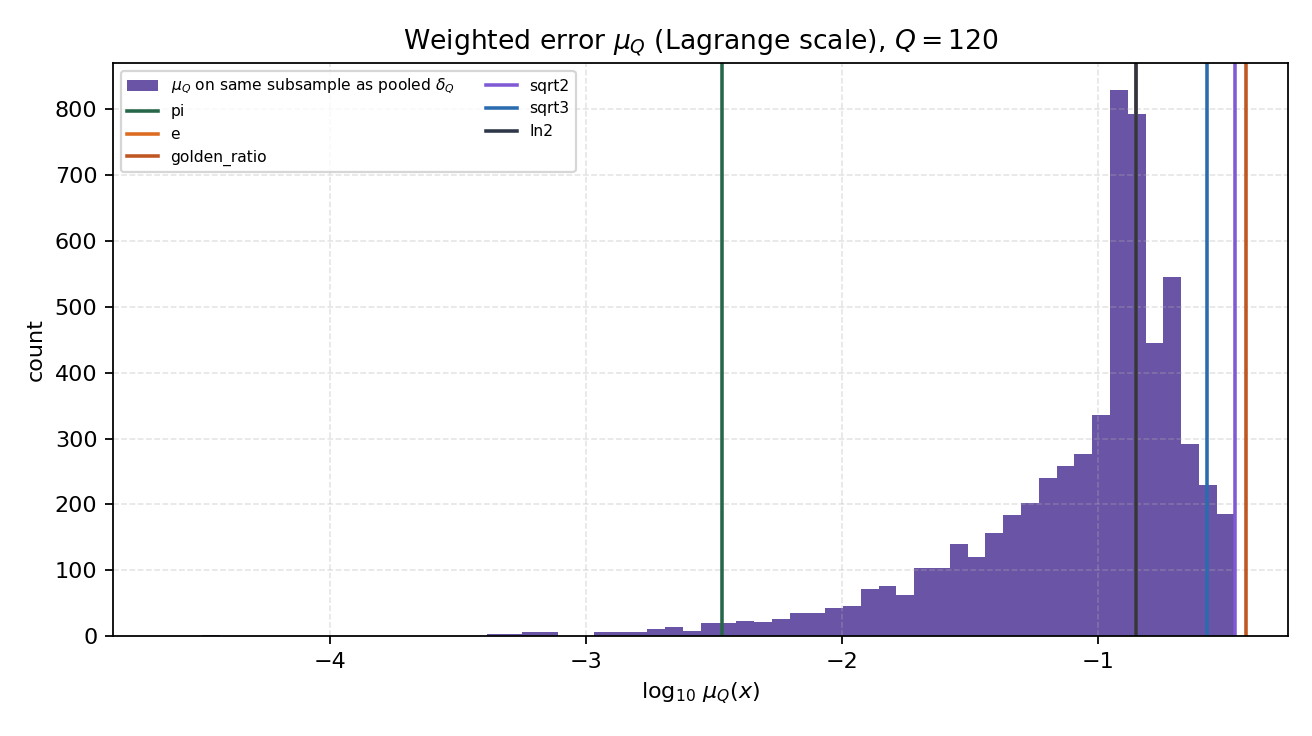
\includegraphics[keepaspectratio,alt={Figure. Histogram of \textbackslash log\_\{10\}\textbackslash mu\_Q(x) on the identical subsample as Figure  (Q=120, same seed and bin count). Vertical lines mark \textbackslash mu\_\{120\}(x\^{}\textbackslash star) for the same six constants. Interpreting this panel alongside Figures -- separates raw closeness \textbackslash delta\_Q from denominator-weighted quality \textbackslash mu\_Q; a constant can sit near the \textbackslash delta\_Q median while lying in an extreme \textbackslash mu\_Q tail if its best admissible approximant is comparatively weak on the q\^{}2 scale.}]{../figures/proximity_histogram_mu.png}}
\caption{\textbf{Figure.} Histogram of \(\log_{10}\mu_Q(x)\) on the
\textbf{identical} subsample as Figure \ref{fig:proximity_pooled}
(\(Q=120\), same seed and bin count). Vertical lines mark
\(\mu_{120}(x^\star)\) for the same six constants. Interpreting this
panel alongside Figures
\ref{fig:proximity_hist}--\ref{fig:proximity_pooled} separates raw
closeness \(\delta_Q\) from denominator-weighted quality \(\mu_Q\); a
constant can sit near the \(\delta_Q\) median while lying in an extreme
\(\mu_Q\) tail if its best admissible approximant is comparatively weak
on the \(q^2\) scale.}\label{fig:proximity_mu}
\end{figure}
\end{block}

\begin{block}{Related checks}
\protect\phantomsection\label{related-checks}
Lattice versus brute-force agreement is recorded in
\texttt{output/data/lattice\_crosscheck.json} from
\texttt{scripts/02\_lattice\_crosscheck.py}.
\end{block}
\end{frame}

\end{document}
